\documentclass[14pt, oneside]{altsu-report}

\worktype{Отчёт по <<Производственная практика: технологическая (проектно-технологическая) практика>> на тему:}
\title{Разработка клеточного автомата <<Игра жизнь>> на платформе Unity}
\author{Б.\,Н.~Ергали}
\groupnumber{5.205-1}
\GradebookNumber{1337}
\supervisor{И.\,А.~Шмаков}
\supervisordegree{ст.пр.}
\ministry{Министерство науки и высшего образования}
\country{Российской Федерации}
\fulluniversityname{ФГБОУ ВО Алтайский государственный университет}
\institute{Институт цифровых технологий, электроники и физики}
\department{Кафедра вычислительной техники и электроники}
\departmentchief{В.\,В.~Пашнев}
\departmentchiefdegree{к.ф.-м.н., доцент}
\shortdepartment{ВТиЭ}


\abstractRU{В отчёте содержатся сведения о курсовой работе.

Курсовая работа заключается в создании кроссплатформенной программы, представляющей Клеточный автомат <<Игра жизнь>>.

В отчёте приведено описание используемой библиотеки Unity, инструментария и системы контроля версий для написания игры на платформе Unity, с использованием языка C \#.

Наряду с этим представлены проверка работспособности программы, диаграмма UML, полный код программы.}
\abstractEN{The report contains information about the course work.

The course work consists of creating a cross-platform program representing the Cellular Automaton <<Game of Life>>.

The report provides a description of the Unity library, tools and version control system used to write a game on the Unity platform using the C\# language.

Along with this, a program functionality test, a UML diagram, and the complete program code are presented.}
\keysRU{программа, игра, пакман, алгоритм, кроссплатформенная программа}
\keysEN{program, game, pacman, algorithm, cross-platform program}

\date{\the\year}

% Подключение файлов с библиотекой.
\addbibresource{graduate-students.bib}

% Пакет для отладки отступов.
%\usepackage{showframe}

\begin{document}
\maketitle

\setcounter{page}{2}
\makeabstract
\tableofcontents

\chapter*{Введение}
\phantomsection\addcontentsline{toc}{chapter}{ВВЕДЕНИЕ}

\textbf{Актуальность:}
Развитие технологий и увеличение доступности программных инструментов для создания игр открывает широкие возможности для исследования сложных систем и процессов через игровую форму. Применение языка программирования \textbf{C\#}~\cite{Cbib} в среде разработки \textbf{Unity}~\cite{un} для создания таких игр объединяет в себе глубокую актуальность как в образовательной, так и в научно-исследовательской сферах.

Создание игры на основе клеточного автомата в среде Unity 2D позволяет не только демонстрировать сложные поведенческие паттерны~\cite{convPat} и взаимодействия между элементами системы в наглядной и доступной форме, но и дает возможность пользователям влиять на процессы внутри игры, экспериментировать с параметрами и наблюдать за их эффектами.

Интерес к созданию собственных миров и экосистем, где каждое действие может привести к непредсказуемым последствиям, высок среди широкой аудитории. Таким образом, разработка игры, основанной на принципах клеточного автомата, является актуальной задачей, способной привлечь внимание как образовательных учреждений, так и широкой публики, интересующейся наукой, технологиями и играми.

\textbf{Цель:}
Создать кроссплатформенный клеточный автомат <<Игра жизнь>> с использованием языка программирования C\#, на платформе Unity.


\textbf{\label{zadachi}Задачи:}
\begin{enumerate}
	\item Изучить платформу Unity.
	\item Изучить алгоритмы клеточных автоматов.
	\item Изучить принцип ООП в C\#.
	\item Изучить сборку проекта в Unity.
        \item Разработать пользовательский интерфейс для взаимодействия с клеточным автоматом.
        \item Провести тестирование и отладку проекта на различных устройствах.
\end{enumerate}

% Подключение первой главы (теория):
\chapter{\label{ch:ch01}ТЕОРЕТИЧЕСКАЯ ЧАСТЬ} % Нужно сделать главу в содержании заглавными буквами

\section{\label{sec:ch01/sec01}Техническое задание}
\begin{enumerate}
	\item Кроссплатформенное приложение, способное запускаться на операционных системах Windows и GNU/Linux.
	\item Написание клеточного автомата <<Игра жизнь>> на платформе Unity, с использованием языка C\#.
	\item Возможность выбора карты.
	\item Возможность генерации случайной карты.
        \item Возможность создания новых карт для клеточного автомата.
	\item Наличие в игре кнопки <<Помощь>>, при нажатии на которую выводится информация о взаимодействии с игрой.
\end{enumerate}

\section{\label{sec:ch01/sec02}Игровой движок}
Для создания кроссплатформенной программы на языке программирования C\# был использован игровой движок Unity

\textbf{Unity} --- это мощная кросс-платформенная среда разработки для создания широкого спектра интерактивного контента, включая видеоигры, обучающие программы, архитектурные визуализации и виртуальную реальность. Она предоставляет интегрированные инструменты для работы как с 2D, так и с 3D-графикой, что делает Unity популярным выбором среди разработчиков игр и интерактивных приложений различного масштаба — от независимых проектов до крупных игровых студий.

Основные особенности и преимущества Unity:
\begin{itemize}
    \item \textbf{Кросс-платформенность:} Unity поддерживает более 25 платформ, включая Windows, macOS, Linux, Android, iOS, WebGL, PlayStation, Xbox и многие другие, что позволяет разработчикам с легкостью портировать свои проекты на различные устройства и экосистемы;
    \item \textbf{Интуитивный интерфейс:} Unity обладает удобным и понятным пользовательским интерфейсом, который упрощает процесс разработки и позволяет даже начинающим разработчикам быстро освоиться в программе.;
    \item \textbf{Мощные инструменты для работы с графикой и анимацией:} В Unity встроены продвинутые инструменты для создания и редактирования 2D и 3D графики, анимаций, а также системы частиц, что делает возможным создание визуально привлекательных и технически сложных проектов;
    \item \textbf{Скриптование на C\#:} Для создания логики игр и приложений в Unity используется язык программирования C\#. Это обеспечивает гибкость и мощь в реализации функционала, делая возможным создание сложных систем взаимодействия и поведения объектов в игровом мире;
    \item \textbf{Активное сообщество и обширная база знаний:} Unity имеет одно из самых больших и активных сообществ разработчиков в мире. Это обеспечивает доступ к огромному количеству учебных материалов, руководств, а также готовых активов и плагинов, которые можно использовать в своих проектах;
    \item \textbf{Unity Asset Store:} Магазин активов Unity предлагает тысячи готовых ресурсов и инструментов, включая модели, текстуры, скрипты, инструменты для интеграции с другими сервисами и многое другое, что значительно ускоряет процесс разработки и позволяет сосредоточиться на уникальных аспектах проекта.
\end{itemize}


\section{\label{sec:ch01/sec03}Инструментарий}
Для написания отчёта с помощью системы компьютерной верстки в \TeX была использована сайт Overleaf.

Для написания кода программы была использована IDE Microsoft Visual Studio.

Для работы с изображениями, используемых в ходе разработки программы, был использован графический редактор Adobe Photoshop 2023~\cite{photoshop}.

Для хранения проекта была выбрана система контроля версия GitHub~\cite{wikiRUGitHub}.

Проверка работоспособности и сборка программы выполнялась на системе:
	\begin{itemize}
		\item \textbf{OC}: \textit{Windows 10}
		\item \textbf{ЦП}: \textit{AMD Ryzen 5 4600H}
		\item \textbf{ОЗУ}: \textit{8gb}
		\item \textbf{Видеокарта}: \textit{NVIDIA GeForce GTX 1650 Ti}
	\end{itemize}

\section{\label{sec:ch01/sec04}Клеточный автомат <<Игра жизнь>>}
\subsection{\label{subsec:ch01/sec04/subsec01}История клеточного автомата <<Игра жизнь>>.}

<<Игра жизнь>> --- это клеточный автомат, созданный британским математиком \textbf{Джоном Конвеем}~\cite{Convei} в 1970 году. Эта <<игра>> стала одним из самых известных примеров клеточного автомата и занимает особое место в теории вычислительных систем и математической биологии.

История создания <<Игры жизнь>> началась с желания Конвея изучить возможности простых математических моделей для имитации жизни и эволюции. Интересно, что, несмотря на простоту правил, <<Игра жизнь>> способна продемонстрировать чрезвычайно сложное и непредсказуемое поведение, что делает ее удивительным примером эмерджентности — появления сложных структур и паттернов из простых взаимодействий. Вместе с коллегами из Кембриджского университета он разработал первые версии игры, которые изначально испытывали на досках для шахмат, заполняя клетки <<живыми>> или <<мертвыми>> состояниями и просчитывая следующие поколения вручную.

Опубликованная в октябре 1970 года в колонке Мартина Гарднера в журнале <<Scientific American>>, <<Игра жизнь>> моментально привлекла внимание широкой аудитории. Люди были поражены идеей, что такие простые правила могут породить бесконечное множество удивительных форм и поведенческих паттернов. В то время как некоторые находили в ней отражение эволюционных процессов и даже возможность изучения искусственного интеллекта, другие видели в <<Игре жизнь>> искусство и новую форму развлечения.

Важной вехой в истории <<Игры жизнь>> стало ее распространение среди первых пользователей персональных компьютеров. Программные реализации игры позволили автоматизировать вычисления и наблюдать за развитием системы в реальном времени, что существенно углубило исследования и способствовало обнаружению всё новых и новых удивительных структур, таких как <<планеры>> (космические корабли), <<планерные пушки>> и самовоспроизводящиеся конструкции.

<<Игра жизнь>> сыграла значительную роль в развитии теории клеточных автоматов и комплексных систем, вдохновив множество ученых и разработчиков на создание собственных моделей и исследования в области искусственной жизни, системной биологии и даже криптографии. Она продолжает оставаться популярной не только среди ученых, но и среди художников, программистов и любителей загадок, представляя собой универсальный язык для исследования сложности из простоты.

\subsection{\label{subsec:ch01/sec04/subsec02}Правила игры}
Правила <<Игры жизнь>> Джона Конвея просты, но в то же время обладают удивительной глубиной, позволяя моделировать сложные динамические процессы. <<Игра>> происходит на бесконечной двумерной сетке клеток, каждая из которых может находиться в одном из двух состояний: быть <<живой>> или <<мертвой>>. Состояние каждой клетки в следующем поколении определяется ее текущим состоянием и состояниями восьми ее соседей по горизонтали, вертикали и диагоналям.

Правила перехода из поколения в поколение следующие:
	\begin{itemize}
		\item \textbf{Рождение}: Мертвая клетка становится живой в следующем поколении, если ровно три из ее восьми соседей живы в текущем поколении. Это правило символизирует репродуктивное <<рождение>> из стабильной, но не перенаселенной среды;
		\item \textbf{Смерть от одиночества}: Живая клетка становится мертвой в следующем поколении, если два или менее из ее восьми соседей живы в текущем поколении. Это моделирует смерть из-за недостатка <<социальных>> взаимодействий;
		\item \textbf{Выживание}: Живая клетка остается живой в следующем поколении, если у нее два или три живых соседа. Это условие обеспечивает оптимальную среду для устойчивого существования;
		\item \textbf{Смерть от перенаселения}: Живая клетка становится мертвой в следующем поколении, если четыре и более из ее восьми соседей живы в текущем поколении. Это представляет смерть из-за слишком высокой конкуренции за ресурсы.
	\end{itemize}

Несмотря на кажущуюся простоту, эти правила порождают удивительно разнообразные и часто непредсказуемые паттерны, включая стационарные фигуры, осциллирующие структуры, которые повторяются через определенное количество поколений, и даже <<космические корабли>>, перемещающиеся по сетке. Эти паттерны и их взаимодействия исследуются в рамках <<Игры жизнь>>, демонстрируя сложность, возникающую из простых начал.


% Подключение второй главы (практическая часть):
\chapter{\label{ch:ch02}ПРАКТИЧЕСКАЯ ЧАСТЬ. ЭТАПЫ РАЗРАБОТКИ ИГРЫ.}

\section{\label{sec:ch02/sec01/sub01}Подготовка и установка окружения.}

Первый шаг на пути к созданию игры — установка \textbf{Unity Hub}~\cite{UnHub}. 

\textbf{Unity Hub} --- это центральное приложение для управления проектами, версиями Unity и лицензиями. 

После установки \textbf{Unity Hub}, можно было начать установку самой платформы \textbf{Unity}. Затем нужно было добавить наиболее стабильную версию \textbf{Unity} и выбрать при необходимости дополнительные компоненты, такие как поддержка различный ОС.

Для написания кода на C\# и работы с Unity была необходима интегрированная среда разработки, или же \textbf{IDE}. Было решено использовать \textbf{Visual Studio}~\cite{vscodeRu}, так как она отлично интегрируется с Unity и предоставляет все необходимые инструменты для разработки. Так как Visual Studio уже был установлен, нужно было дополнительно к нему загрузить рабочую нагрузку \textbf{Game development with Unity}~\cite{vsUn}. Это обеспечило установку всех нужных компонентов для работы с Unity и написания кода на C\#.

После установки всех необходимых инструментов был создан новый проект в Unity. В выборе шаблона проекта, выбор пал на 2D, т.к. необходимости в 3D пространстве не было и все можно было выполнить в 2D. 

Перед началом работы непосредственно с самим редактором Unity, необходимо было ознакомиться с интерфейсом и основными инструментами, необходимыми для разработки, т.к. изначально интерфейс мог казаться перегруженным различными панелями и кнопками. 

Основные инструменты разработки которые следовало изучить, были панели инструментов (см. рисунок~\ref{fig4}). : 
	\begin{itemize}
		\item Панель \textbf{Hierarchy} (1) показывает все объекты, находящиеся в текущей сцене.
		\item Панель \textbf{Scene} (2) позволяет визуально редактировать сцену. 
		\item Панель \textbf{Game} (3) используется для предпросмотра игры. 
		\item Панель \textbf{Inspector} (4) позволяет настраивать свойства выбранного объекта.
            \item Панель \textbf{Project} (5) помогает управлять файлами и папками проекта
            \item Панель \textbf{Console} (6) выводит ошибки, предупреждения и сообщения отладки.
	\end{itemize}

\begin{figure}[H]
	\centering
	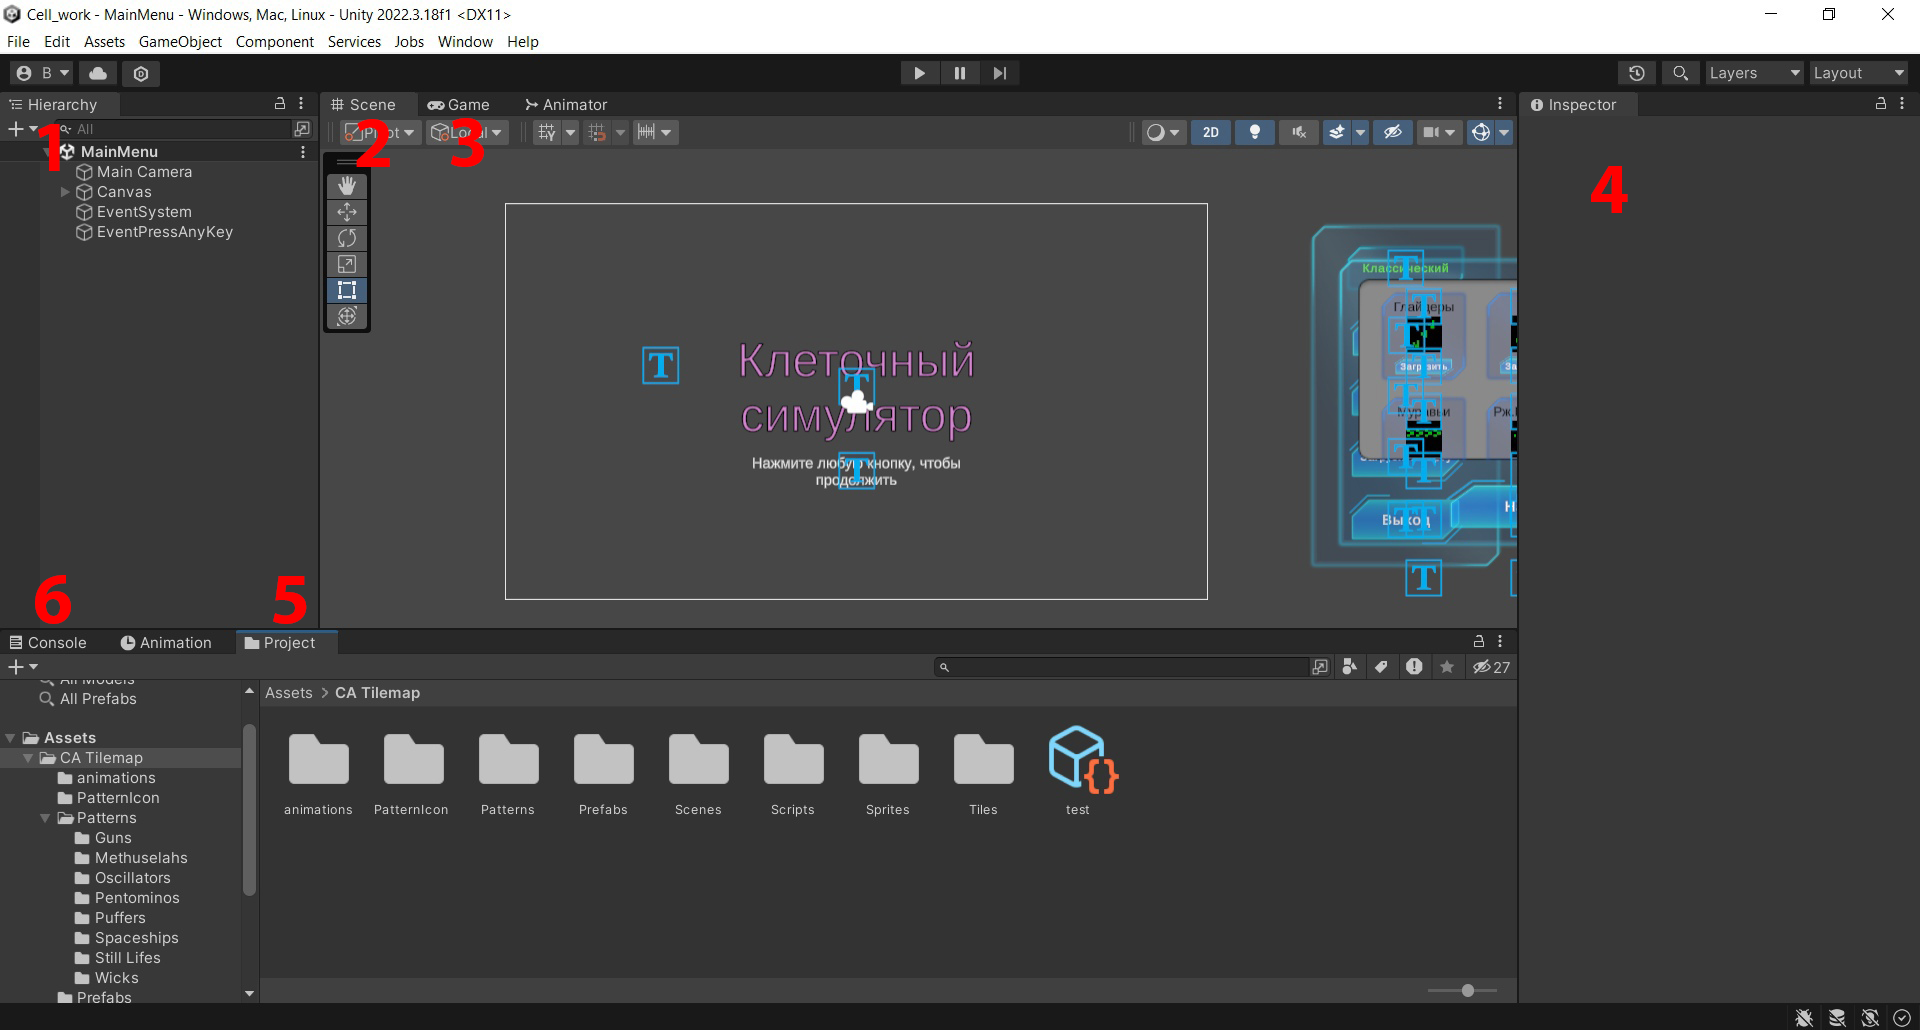
\includegraphics[width=1\textwidth]{images/Panels.png}  
	\caption{Панели инструментов.}
	\label{fig4}
\end{figure}

Далее появилась необходимость в изучении теории~\cite{OsnUnity}. В Unity есть несколько ключевых понятий, которые важно понимать с самого начала, т.к. большинство форумов и книг используют их. К ним относятся такие понятия как:
	\begin{itemize}
		\item \textbf{GameObject} --- это базовый объект в Unity, к которому можно прикреплять различные компоненты, такие как скрипты, физические свойства или визуальные элементы.
		\item \textbf{Component} --- это то, что добавляется к GameObject для придания ему различных свойств и функциональностей. 
		\item\textbf{Scene} --- это пространство, в котором располагаются все GameObjects. Игра может состоять из нескольких сцен, например, меню, уровня и экрана победы. 
		\item \textbf{Prefab} --- это шаблон объекта, который можно многократно использовать в проекте.
	\end{itemize}

После ознакомления с интерфейсом и основными понятиями, был сделан вывод, что рабочий стол организован и все необходимые инструменты настроены, что значительно упростило дальнейшую работу и позволило сосредоточиться на создании проекта.

\section{\label{sec:ch02/sec01/sub02}Реализация основного алгоритма клеточного автомата.}

После подготовки и установки окружения была выполнена реализация базового алгоритма клеточного автомата. Этот алгоритм представляет собой математическую модель, которая имитирует поведение клеток на двумерной решетке. Каждая клетка может быть либо <<живой>>, либо <<мертвой>>, и её состояние в следующем поколении зависит от состояния соседних клеток.

Вначале было проведено теоретическое изучение основных правил <<Игры жизни>>~\cite{GameLife}. Эти правила включали в себя: смерть клетки от одиночества при наличии менее двух живых соседей, выживание при двух или трёх живых соседях, смерть от перенаселения при наличии более трёх живых соседей и возрождение мёртвой клетки при наличии ровно трёх живых соседей.

После этого началась разработка алгоритма. В Unity был создан скрипт на языке C\#, который реализовывал логику обновления состояния клеток. Вместо использования классического двумерного массива, был использован массив, хранящий координаты клеток из \textbf{Tilemap}~\cite{tilemap}. Это позволило учитывать специфические особенности Unity и обеспечить более точное взаимодействие с визуальной частью игры. В ходе разработки использовался скрипт \textbf{GameBoard.cs}(см. \textbf{\textsc{ПРИЛОЖЕНИЕ}} на стр.~\pageref{code:brgame}), в котором хранилась логика основной симуляции. В этом скрипте были В функции \textbf{UpdateState()}(см. \textbf{\textsc{ПРИЛОЖЕНИЕ}} на стр.~\pageref{code:brgame} строки 118-164) в котором происходило обновление их состояния и визуализации текущего состояния на \textbf{Tilemap}, а функция \textbf{SetPattern()}(см. \textbf{\textsc{ПРИЛОЖЕНИЕ}} на стр.~\pageref{code:brgame} строки 66-82) отвечала за начальную настройку массива клеток случайными значениями.  В частности, использовались методы для определения состояния клетки и её соседей, такие как \textbf{IsAlive()} и \textbf{CountNeighbors()}(см. \textbf{\textsc{ПРИЛОЖЕНИЕ}} на стр.~\pageref{code:brgame} строки 210-213 и строки 166-198).

\textbf{Tilemap} в Unity оказался удобным инструментом для визуализации клеточного автомата. Это компонент, который позволяет легко создавать и редактировать двумерные сетки, используя тайлы (маленькие графические элементы). Для визуализации состояния клеток был создан новый \textbf{Tilemap} в сцене Unity. Этот компонент позволил упрощённое отображение и управление клетками на игровом поле.



Был написан скрипт \textbf{TilemapClickHandler.cs}(см. \textbf{\textsc{ПРИЛОЖЕНИЕ}} на стр.~\pageref{code:click}), который обеспечивал взаимодействие с клетками на уровне визуализации. Этот скрипт позволял пользователю кликать по клеткам, тем самым создавая их, что делало игровой опыт более интерактивным и удобным и в то же время демонстрировала работу алгоритма.

Во время тестирования и отладки были выявлены несколько проблем. Например, неправильное определение количества соседей у граничных клеток и ошибки при копировании массивов, что приводило к некорректному обновлению состояния клеток. Эти проблемы были исправлены в ходе тщательной отладки кода. Были также внедрены различные методы для проверки корректности работы алгоритма и его соответствия правилам <<Игры жизни>>.

Для обеспечения плавной работы алгоритма на разных устройствах была проведена оптимизация кода. Основное внимание уделялось минимизации количества операций в основном цикле обновления, использованию эффективных методов для копирования и обновления массивов, а также оптимизации рендеринга клеток. В результате проведённых оптимизаций алгоритм стал работать более плавно и эффективно, даже при увеличении размера поля и частоты обновления.

Таким образом алгоритм клеточного автомата <<Игры жизни>> был реализован, протестирован и визуализирован с использованием Tilemap, что позволило перейти к следующим этапам разработки проекта.

\section{\label{sec:ch02/sec01/sub03}Создание пользовательского интерфейса (UI)}

После реализации и проверки основной механики игры, началось выполнение этапа разработки пользовательского интерфейса (UI) для игры <<Игра жизни>>. 
Этот этап включал в себя создание интерактивных элементов, которые позволяли пользователям управлять симуляцией, редактировать, загружать и генерировать их, а также изменять параметры клеточного автомата. Основной задачей было сделать интерфейс интуитивно понятным и удобным для пользователя.

Для обеспечения удобства использования и отзывчивости интерфейса были изучены и применены практики UI/UX-дизайна~\cite{UI/Ux}, чтобы интерфейс был интуитивно понятным и легко читаемым. Особое внимание было уделено размеру и расположению кнопок, а также цветовой гамме интерфейса.

Для начала было решено создать основные элементы управления симуляцией. В Unity на главном экране игры было разработано основное меню, которое включало несколько ключевых кнопок:
        \begin{itemize}
		\item \textbf{Редактор} --- переход в режим редактирования клеточного автомата..
		\item \textbf{Случайная генерация} --- создание случайного начального состояния. 
		\item\textbf{Загрузить карту} --- загрузка предварительно сохраненных паттернов. 
		\item \textbf{Выход} --- завершение работы программы.
            \item \textbf{Помощь} --- загрузка описания проекта и автора.
	\end{itemize}

Эти элементы управления были реализованы с использованием стандартных UI-компонентов Unity, таких как Button и Panel.

Первым делом для удобства пользователей была создана отдельная панель, где можно было выбрать предопределенные паттерны клеток. На этой панели отображались кнопки с изображениями и названиями паттернов, таких как Глайдеры, Иви, Блинкер, Муравьи, Ружье Госпера и Вакуумная пушка~\cite{pattern}. Пользователь мог загрузить выбранный паттерн, нажав соответствующую кнопку <<Загрузить>>. Эта функциональность была реализована с помощью скрипта \textbf{LevelTransition.cs} (см. \textbf{\textsc{ПРИЛОЖЕНИЕ}} на стр.~\pageref{code:lvl})

Следом была создана отдельная панель, где пользователь мог задать размер карты и случайным образом сгенерировать начальное состояние клеток. На этой панели размещались кнопки для выбора размеров карты (20x20, 50x50, 100x100) и кнопка <<Сгенерировать>>, которая инициализировала случайное распределение живых клеток на карте. Эта функциональность была реализована с помощью скрипта \textbf{RandomButton.cs}. (см. \textbf{\textsc{ПРИЛОЖЕНИЕ}} на стр.~\pageref{code:rndB}). 

Для режима редактирования была создана отдельная сцена где пользователь мог задать размер карты перед началом редактирования и так же для интерактивного управления клетками была реализована возможность изменения состояния клеток с помощью кликов мыши. Эта функциональность была реализована с помощью скриптов \textbf{TilemapClickHandler.cs} и \textbf{EditorStartMap.cs}. (см. \textbf{\textsc{ПРИЛОЖЕНИЕ}} на стр.~\pageref{code:strMap})

После разработки основных элементов интерфейса было проведено тщательное тестирование. Были выявлены и исправлены ошибки, связанные с отображением информации и взаимодействием с элементами управления. Тестирование проводилось на различных устройствах, чтобы убедиться в корректной работе интерфейса на всех поддерживаемых разрешениях.


\section{\label{sec:ch02/sec01/sub04}Блок-схема.}

Блок-схема <<Игры жизни>> Джона Конвея иллюстрирует процесс обновления состояния клеток на игровом поле. Алгоритм основан на простых правилах, которые определяют, будет ли клетка <<живой>> или <<мертвой>> в следующем поколении, в зависимости от состояния её соседей. Данная блок-схема показывает основные этапы работы алгоритма, начиная с инициализации и заканчивая обновлением состояния клеток (см. рисунок~\ref{fig4}). 

\begin{figure}[H]
	\centering
	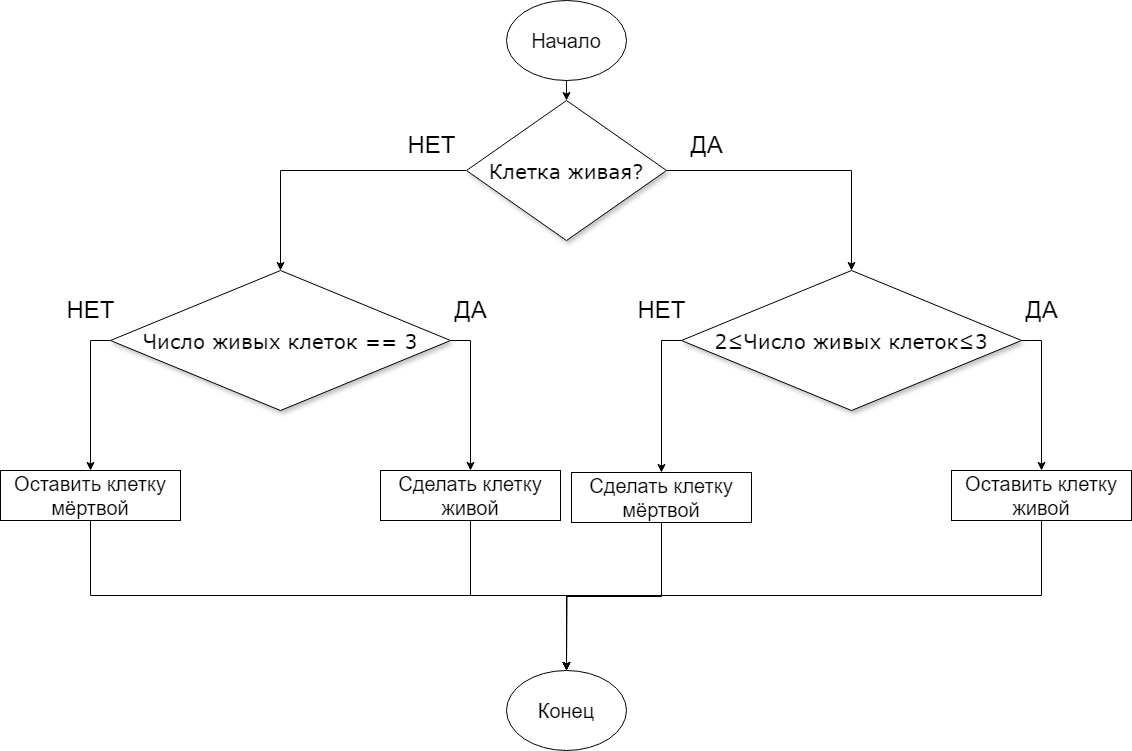
\includegraphics[width=1\textwidth]{images/БлокСхема.png}  
	\caption{Блок схема алгоритма <<Игры жизни>>.}
	\label{fig4}
\end{figure}

\section{\label{sec:ch02/sec01/sub05}Сборка программы}

Сборка программы является предфинальным этапом разработки проекта в Unity. На этом этапе проект подготавливается к запуску на различных платформах, таких как Windows, macOS, Linux, iOS и других. В данном разделе описаны шаги по сборке программы, начиная с настройки проекта и заканчивая созданием исполняемых файлов.

Перед сборкой программы необходимо было убедиться, что все параметры проекта настроены правильно. Для этого в Unity используется меню <<File > Build Settings...>>. В открывшемся окне можно выбрать платформу, на которую будет производиться сборка, а также настроить основные параметры.

\begin{figure}[H]
	\centering
	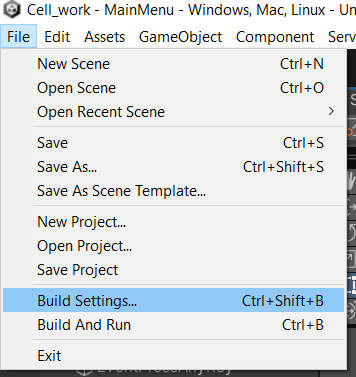
\includegraphics[width=1\textwidth]{images/build1.png}  
	\caption{Открытие меню Build Settings.}
	\label{fig5}
\end{figure}

В окне <<Build Settings>> выберется платформа, на которую будет производиться сборка (например, PC, Mac \& Linux Standalone для Windows и macOS, или Android для мобильных устройств). Были добавлены все необходимые сцены в раздел <<Scenes In Build>>, нажав на кнопку <<Add Open Scenes>>. Необходимо было убедитесь, что все сцены, которые должны быть включены в сборку, добавлены в этот список.

\begin{figure}[H]
	\centering
	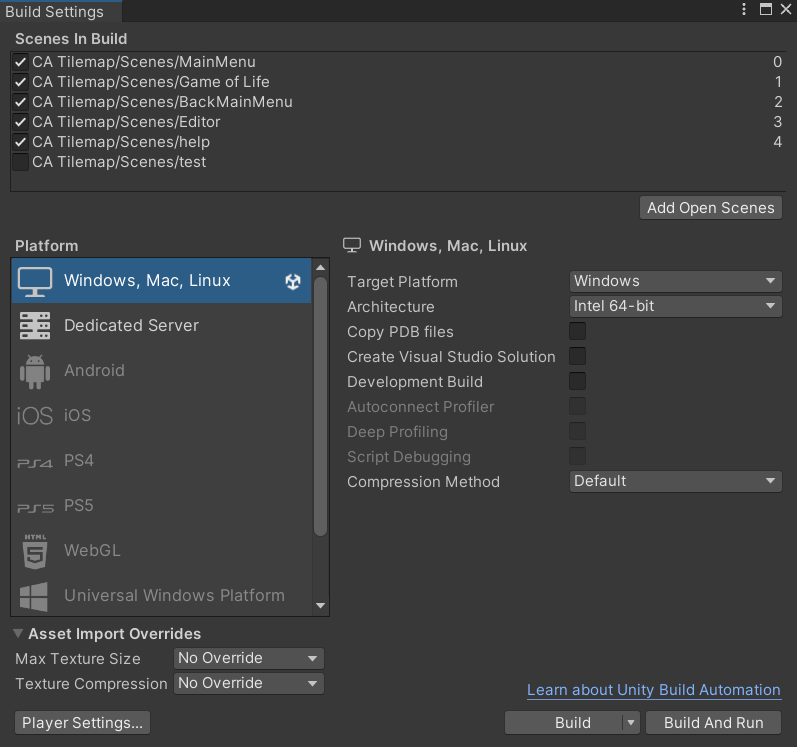
\includegraphics[width=1\textwidth]{images/build2.png}  
	\caption{Окно Build Settings.}
	\label{fig5}
\end{figure}

В зависимости от выбранной платформы могут потребоваться дополнительные настройки. Для Windows и macOS также можно было настроить параметры отображения, значки и другие параметры.

После настройки всех параметров нажав на кнопку <<Build>>, Unity предложило выбрать папку, в которую будет сохранен скомпилированный проект.Выбрав подходящее место, начался процесс сборки.

Скомпилированным проект в папке будет иметь такой вид (см. рисунок~\ref{fig5}). 
\begin{figure}[H]
	\centering
	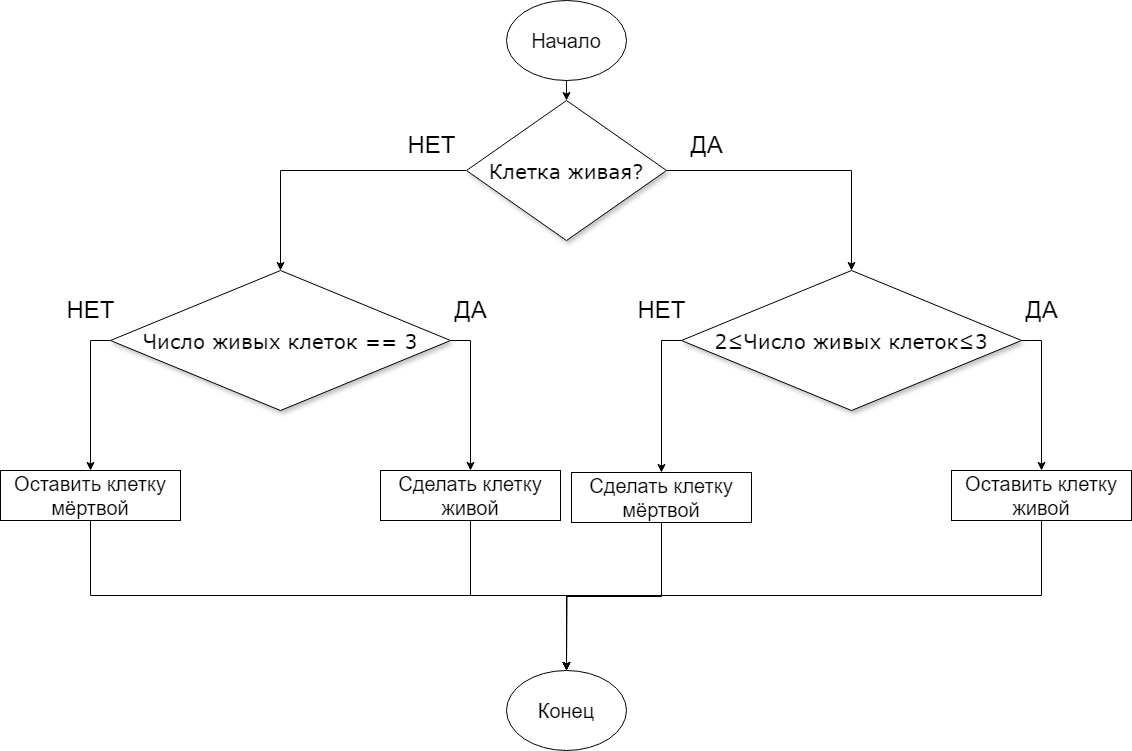
\includegraphics[width=1\textwidth]{images/БлокСхема.png}  
	\caption{Блок схема алгоритма <<Игры жизни>>.}
	\label{fig5}
\end{figure}

\section{\label{sec:ch02/sec01/sub06}Тестирование программы}

После завершения сборки в конце необходимо было протестировать скомпилированный проект на целевой платформе. Запустить созданный исполняемые файлы на соответствующей операционной системе и следовало убедиться, что программа работает корректно. Проверив все основные функции и элементы интерфейса, убедиться в отсутствии ошибок. 

При запуске игры нас встречает главное меню (см. \textbf{\textsc{ПРИЛОЖЕНИЕ}} на стр.~\pageref{MainM}).

При нажатии на кнопку <<Редактор>> меняется экран. На нём отображена возможность редактирования игрового поля и задания размеров карты (см. \textbf{\textsc{ПРИЛОЖЕНИЕ}} на стр.~\pageref{Editor}). 

При нажатии на кнопку <<Случайная Генерация>> появляется панель. На ней отображены настройки размера карты (см. \textbf{\textsc{ПРИЛОЖЕНИЕ}} на стр.~\pageref{rand}). 

При нажатии на кнопку <<Загрузить карту>> появляется панель. На ней отображены кнопки выбора предопределенных паттернов и загрузки карты (см. \textbf{\textsc{ПРИЛОЖЕНИЕ}} на стр.~\pageref{downl}). 

Основное игровое поле выглядит следующим образом (см. \textbf{\textsc{ПРИЛОЖЕНИЕ}} на стр.~\pageref{map}).

Пример ситуации, когда запускается симуляция <<Игры жизни>>, некоторые клетки появляются, исчезают или остаются неизменными в зависимости от правил, приведены ниже (см. \textbf{\textsc{ПРИЛОЖЕНИЕ}} на стр.~\pageref{uim}).

% Подключение третий главы (практическая часть с тестированием:

\chapter*{Заключение}
\phantomsection\addcontentsline{toc}{chapter}{ЗАКЛЮЧЕНИЕ}
В ходе выполнения лабораторной работы была создана кроссплатформенная программа с использованием языка программирования C\# и платформы Unity.

Программа создавалась в объектно-ориентированной парадигме.

Программа представляет собой симулятор клеточного автомата <<Игра жизни>>.

Кнопки, экраны <<Помощь>>, <<Редактор>>, <<Случайная генерация>>, <<Загрузить карту>>, <<Выход>> – все эти объекты были добавлены в программу. Кнопки срабатывают при нажатии на них, при этом меняется экран. Выбор размеров карты и типов начальных паттернов успешно выполняется. Симуляция запускается соответствующими кнопками. Все взаимодействия между пользователем и игровым полем успешно отрабатываются.

Программы выполнена в соответствии с \textbf{\textsc{Техническим заданием}} на странице~\pageref{sec:ch01/sec01}.

Были решены все поставленные задачи (см. \textbf{\textsc{Задачи}} на стр.~\pageref{zadachi}).

Разработка программы и отчёта производилась с использованием системы контроля версий Git~\cite{git}, а конкретнее с помощью онлайн-хранилища GitHub.

По коду программы была создана блок-схема (см. на стр.~\pageref{fig5}.

Была успешна выполнена сборка игры под операционную систему Microsoft Windows (см. \textbf{\textsc{Сборка программы}} на стр.~\pageref{sec:ch02/sec01/sub06}).

Проверка работоспособности программы была проведена успешно (см. \textbf{\textsc{Проверка работоспособности программы}} на стр.~\pageref{sec:ch02/sec01/sub7}).

Отчёт оформлен с помощью системы компьютерной вёрстки \TeX{} и его расширения \XeTeX{} из дистрибутива \textit{TeX Live}.

Ссылка на репозиторий проекта:~\textcolor{blue}{\url{https://github.com/KapKanZhan/Game-Life-Coursework.git}}

\newpage
\phantomsection\addcontentsline{toc}{chapter}{СПИСОК ИСПОЛЬЗОВАННОЙ ЛИТЕРАТУРЫ}
\printbibliography[title={СПИСОК ИСПОЛЬЗОВАННОЙ ЛИТЕРАТУРЫ}]

\appendix
\newpage
\chapter*{\raggedleft\label{appendix1}ПРИЛОЖЕНИЕ}
\phantomsection\addcontentsline{toc}{chapter}{ПРИЛОЖЕНИЕ}
%\section*{\centering\label{code:appendix}Текст программы}



\begin{center}
\label{code:appendix}Текст программы
\end{center}



\begin{code}
\captionof*{listing}{\centering\label{code:brgame}Основной скрипт инициализации карты и алгоритма игры}
\vspace{-1cm}\inputminted[mathescape,linenos,frame=lines,fontsize=\tiny,breaklines]{csharp}{src/GameBoard.cs}
\end{code}

\begin{code}
\captionof*{listing}{\centering\label{code:click}Скрипт создания клеток по клику мыши}
\vspace{-1cm}\inputminted[mathescape,linenos,frame=lines,fontsize=\tiny,breaklines]{csharp}{src/TilemapClickHandler.cs}
\end{code}

\begin{code}
\captionof*{listing}{\centering\label{code:pi-example}Скрипт возвращения в главное меню}
\vspace{-1cm}\inputminted[mathescape,linenos,frame=lines,fontsize=\tiny,breaklines]{csharp}{src/BackMainMenu.cs}
\end{code}

\begin{code}
\captionof*{listing}{\centering\label{code:pi-example}Скрипт возвращения в главное меню}
\vspace{-1cm}\inputminted[mathescape,linenos,frame=lines,fontsize=\tiny,breaklines]{csharp}{src/BackMainMenu.cs}
\end{code}

\begin{code}
\captionof*{listing}{\centering\label{code:pi-example}Скрипт отрисовки границ карты}
\vspace{-1cm}\inputminted[mathescape,linenos,frame=lines,fontsize=\tiny,breaklines]{csharp}{src/BorderDraw.cs}
\end{code}

\begin{code}
\captionof*{listing}{\centering\label{code:pi-example}Скрипт динамической камеры}
\vspace{-1cm}\inputminted[mathescape,linenos,frame=lines,fontsize=\tiny,breaklines]{csharp}{src/CameraAdjuster.cs}
\end{code}

\begin{code}
\captionof*{listing}{\centering\label{code:pi-example}Скрипт перехода на сцену редактирования}
\vspace{-1cm}\inputminted[mathescape,linenos,frame=lines,fontsize=\tiny,breaklines]{csharp}{src/EditorButton.cs}
\end{code}

\begin{code}
\captionof*{listing}{\centering\label{code:strMap}Скрипт запуска созданной карты в режиме редактирования}
\vspace{-1cm}\inputminted[mathescape,linenos,frame=lines,fontsize=\tiny,breaklines]{csharp}{src/EditorStartMap.cs}
\end{code}

\begin{code}
\captionof*{listing}{\centering\label{code:pi-example}Скрипт выхода из игры}
\vspace{-1cm}\inputminted[mathescape,linenos,frame=lines,fontsize=\tiny,breaklines]{csharp}{src/ExitButton.cs}
\end{code}

\begin{code}
\captionof*{listing}{\centering\label{code:pi-example}Скрипт создания паттерна}
\vspace{-1cm}\inputminted[mathescape,linenos,frame=lines,fontsize=\tiny,breaklines]{csharp}{src/Pattern.cs}
\end{code}

\begin{code}
\captionof*{listing}{\centering\label{code:pi-example}Скрипт выключения заставки}
\vspace{-1cm}\inputminted[mathescape,linenos,frame=lines,fontsize=\tiny,breaklines]{csharp}{src/PressAnyKey.cs}
\end{code}

\begin{code}
\captionof*{listing}{\centering\label{code:pi-example}Скрипт выключения заставки по нажатию любой кнопки}
\vspace{-1cm}\inputminted[mathescape,linenos,frame=lines,fontsize=\tiny,breaklines]{csharp}{src/PressAnyKey.cs}
\end{code}

\begin{code}
\captionof*{listing}{\centering\label{code:rndB}Скрипт генерации и запуска карты в режиме Случайная Генерация}
\vspace{-1cm}\inputminted[mathescape,linenos,frame=lines,fontsize=\tiny,breaklines]{csharp}{src/RandomButton.cs}
\end{code}

\begin{code}
\captionof*{listing}{\centering\label{code:lvl}Скрипт готового паттерна в режиме Загрузить Карту}
\vspace{-1cm}\inputminted[mathescape,linenos,frame=lines,fontsize=\tiny,breaklines]{csharp}{src/LevelTransition.cs}
\end{code}

\begin{figure}[H]
	\centering
	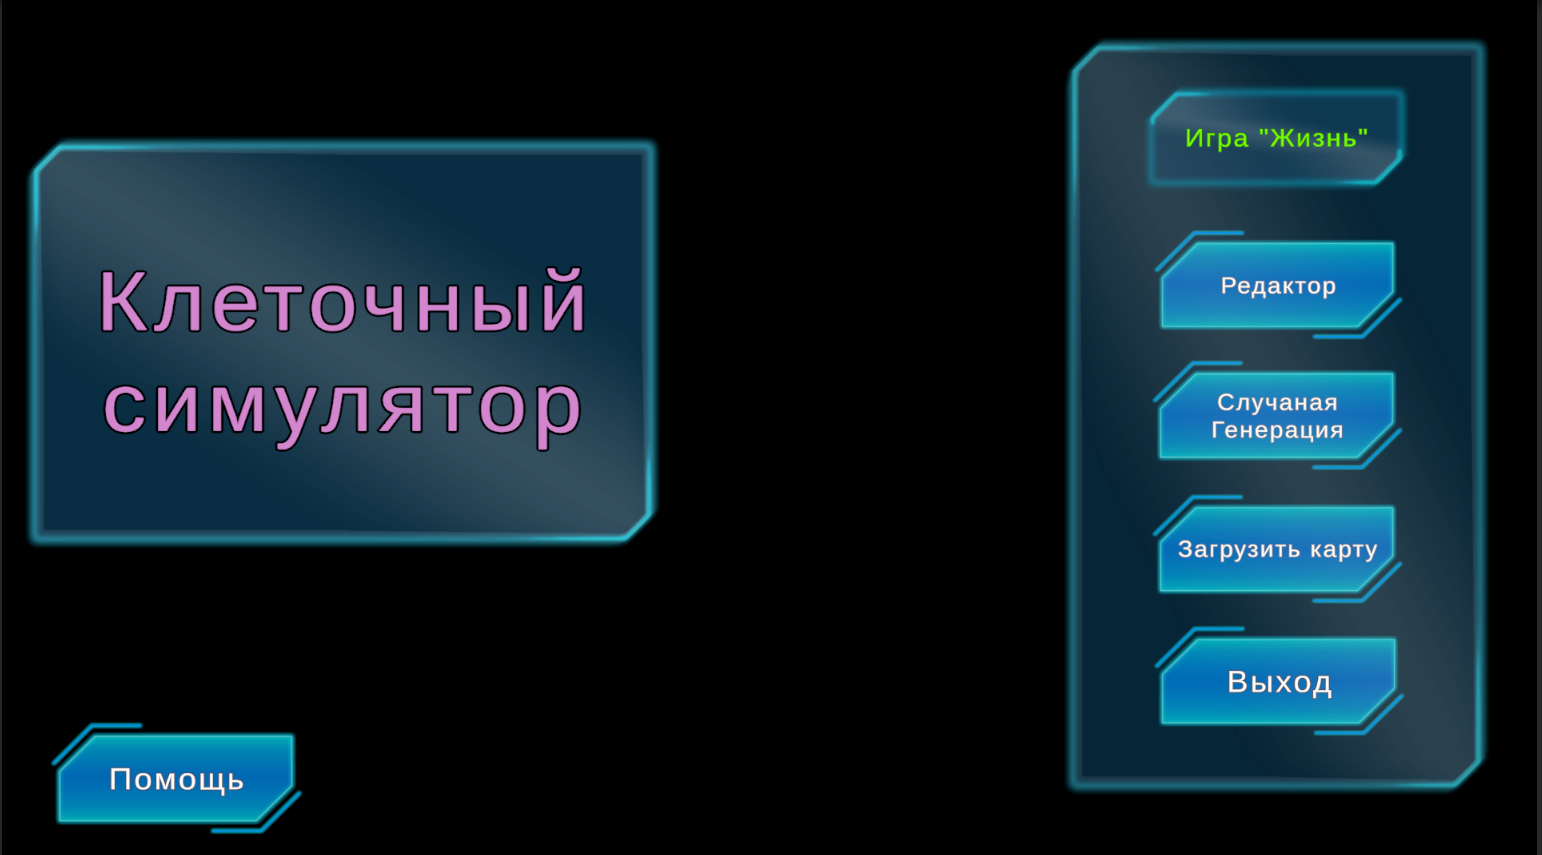
\includegraphics[width=1\textwidth]{images/MainMenu.png}  
	\caption{Главное меню <<Игры жизнь>>.}
	\label{MainM}
\end{figure}

\begin{figure}[H]
	\centering
	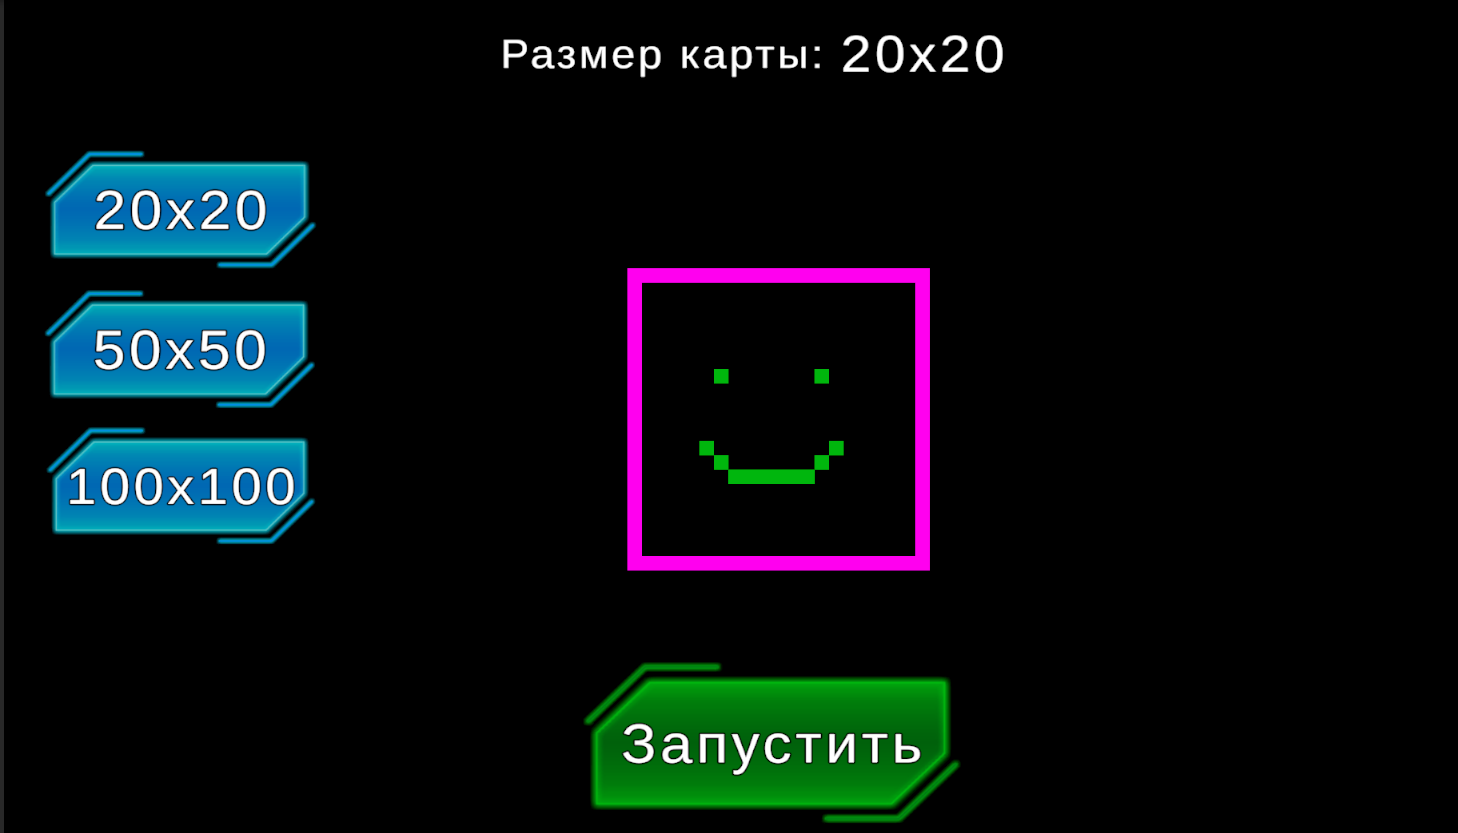
\includegraphics[width=1\textwidth]{images/Editor.png}  
	\caption{Редактор.}
	\label{Editor}
\end{figure}

\begin{figure}[H]
	\centering
	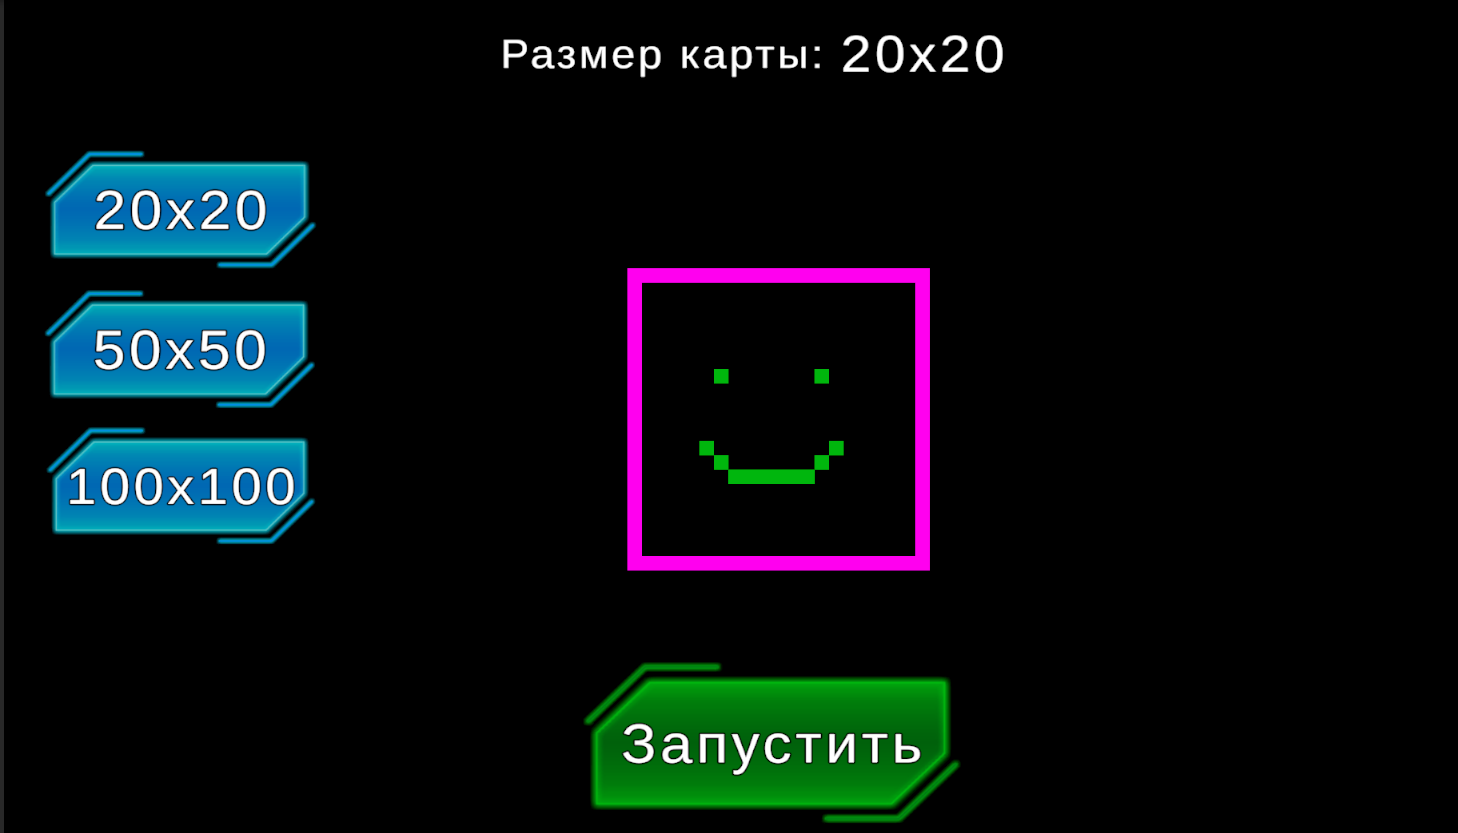
\includegraphics[width=1\textwidth]{images/Editor.png}  
	\caption{Окно редактора.}
	\label{Editor}
\end{figure}

\begin{figure}[H]
	\centering
	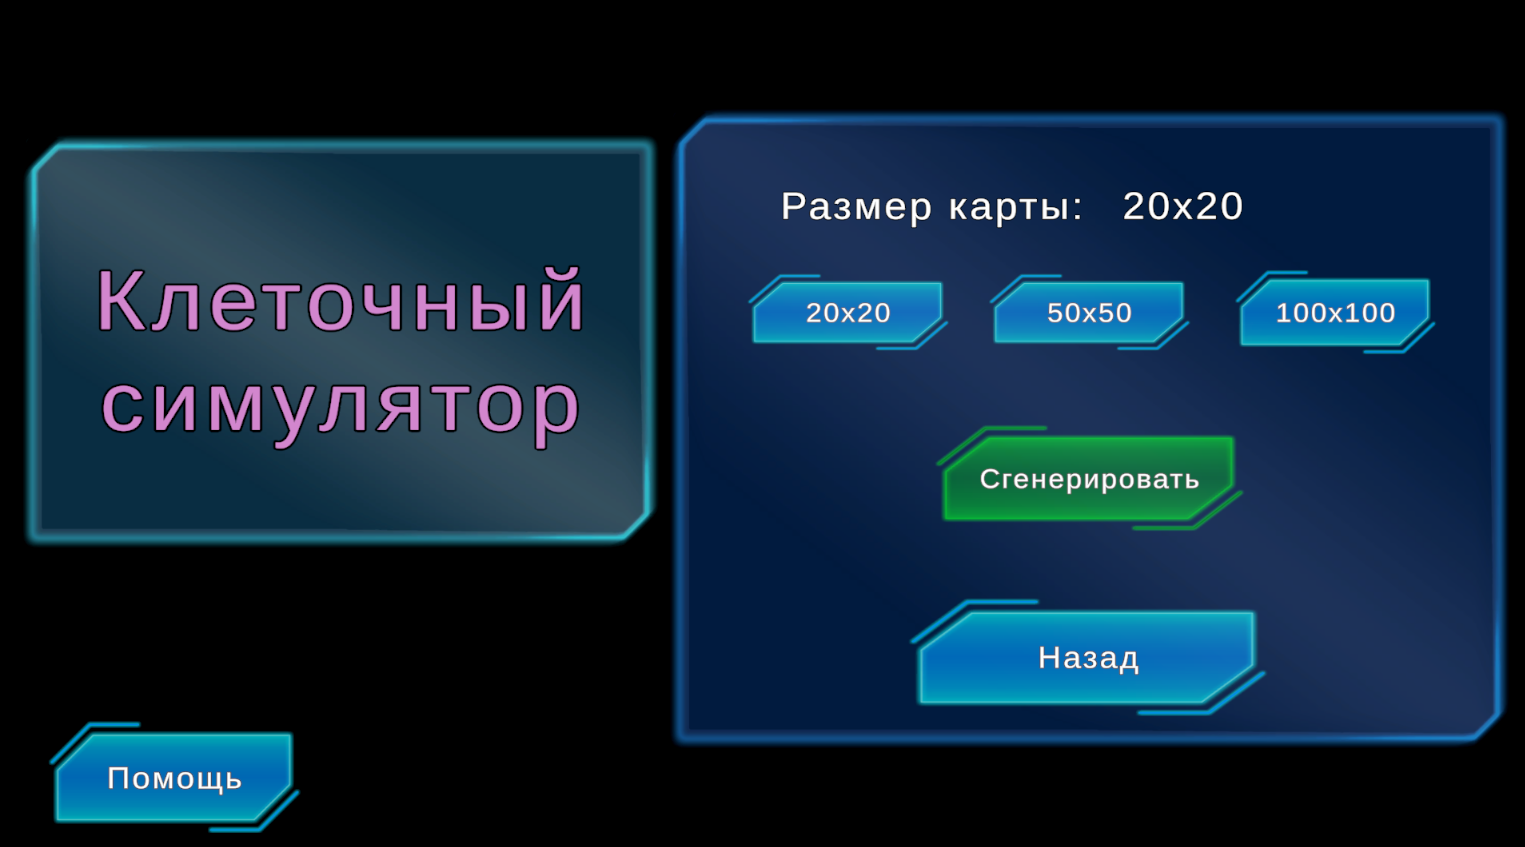
\includegraphics[width=1\textwidth]{images/rand1.png}  
	\caption{Панель Случайной генерации.}
	\label{rand}
\end{figure}

\begin{figure}[H]
	\centering
	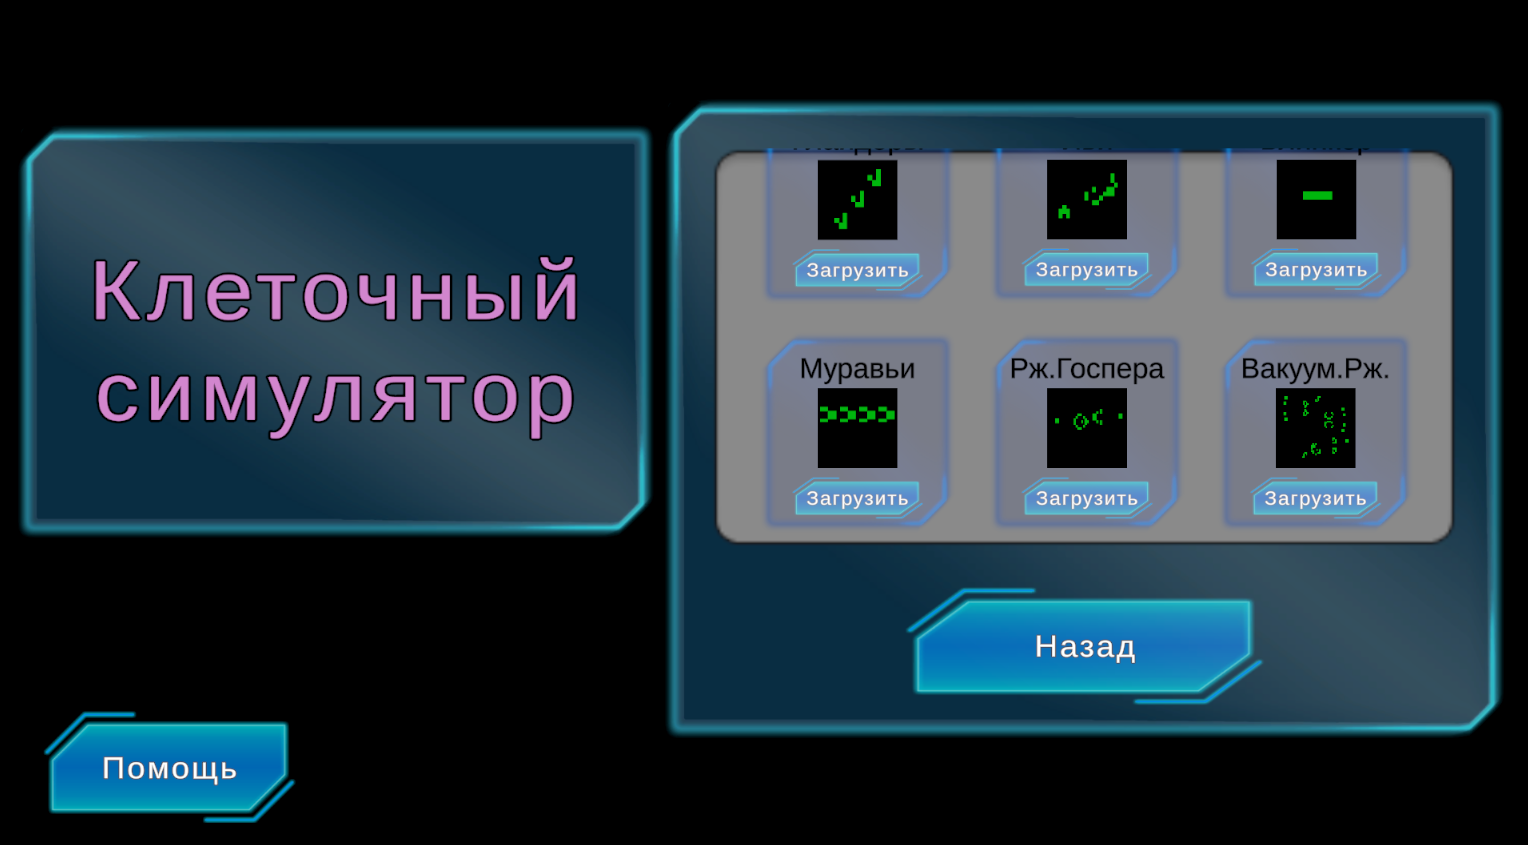
\includegraphics[width=1\textwidth]{images/downld.png}  
	\caption{Панель Загрузки карт.}
	\label{downl}
\end{figure}

\begin{figure}[H]
	\centering
	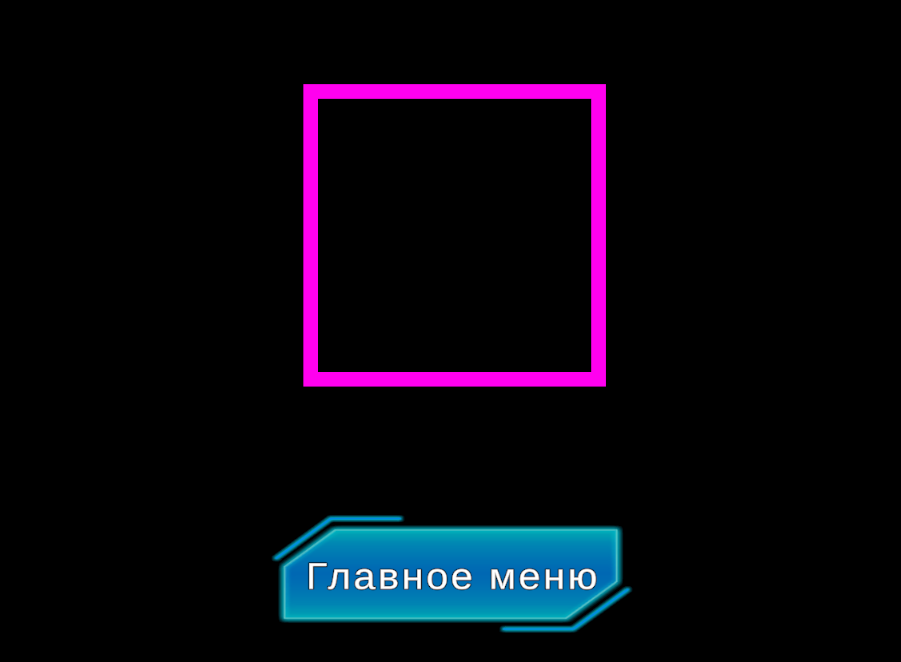
\includegraphics[width=1\textwidth]{images/map.png}  
	\caption{Игровое поле.}
	\label{map}
\end{figure}

\begin{figure}[H]
	\centering
	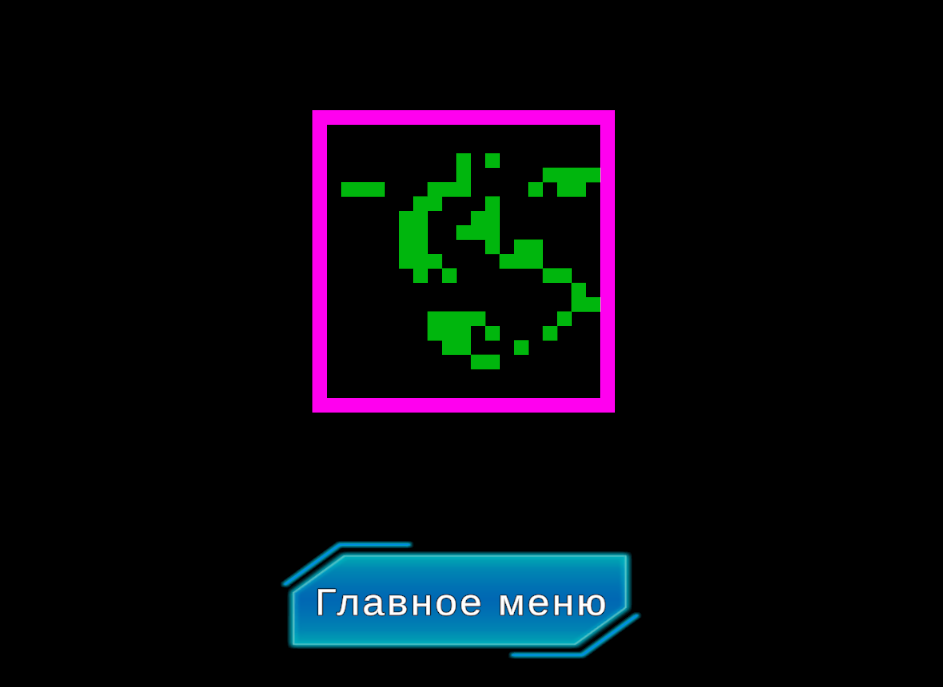
\includegraphics[width=1\textwidth]{images/rand2.png}  
	\caption{Симуляция.}
	\label{uim}
\end{figure}

\end{document}

